\chapter{Georeferencing}
\section{Georeferencing with point cloud}

It is possible to set session as ground truth.
Thus, optimization process (Pose GRAPH SLAM) will not change its poses.
Other sessions can be aligned against ground truth session by adding edges.

\begin{figure}[H]
	\centering
	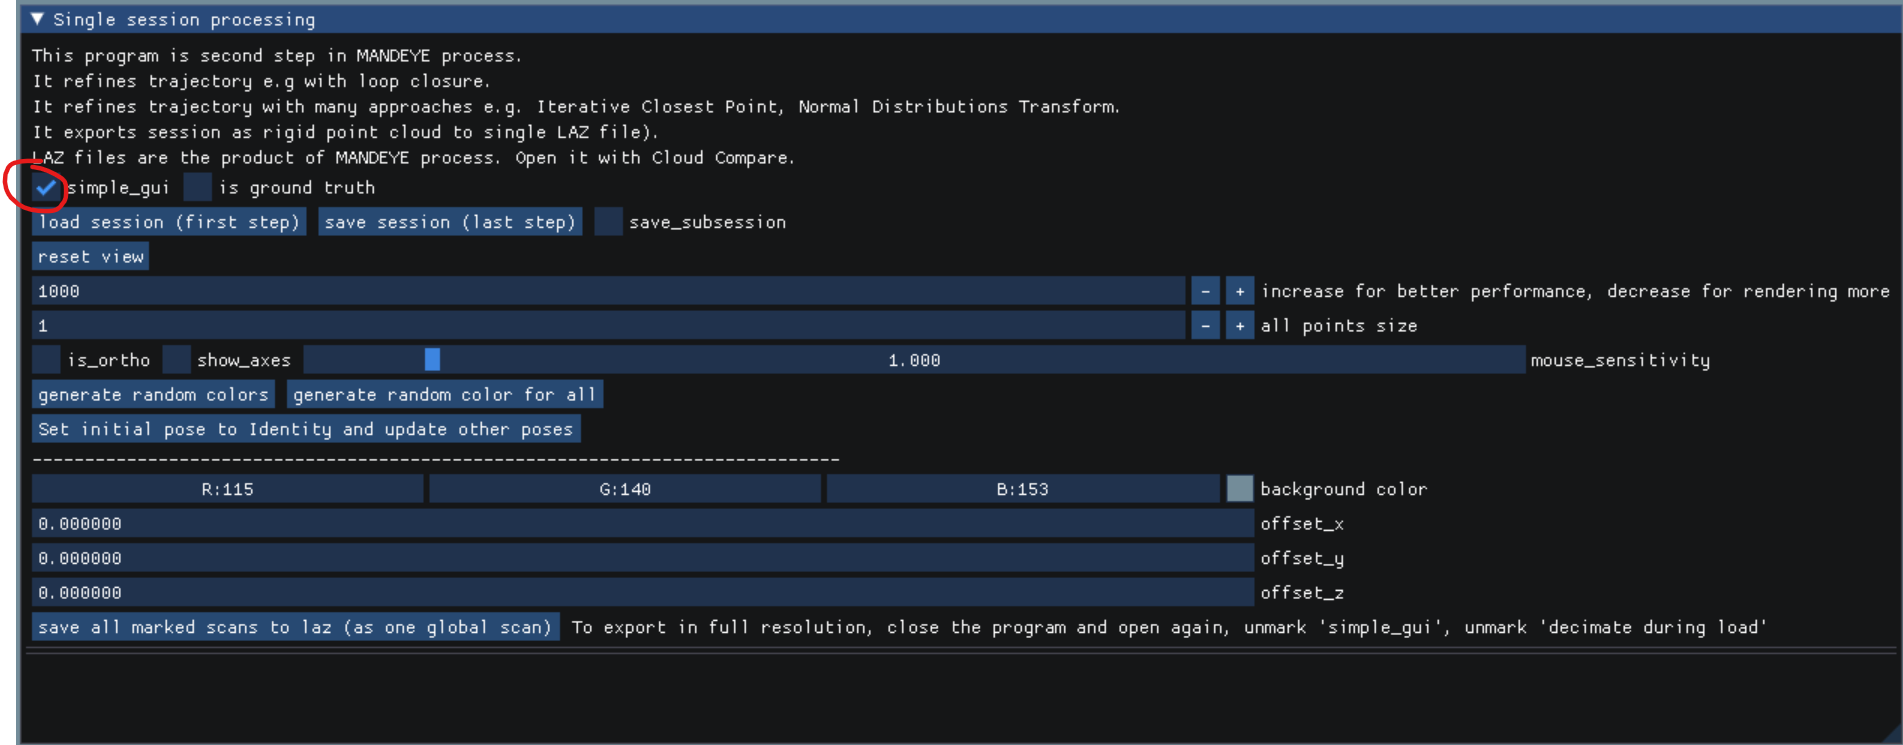
\includegraphics[width=\textwidth]{g1.png}
	\caption{Use multi view tls registration step2 program to open TLS files.}
	\label{fig:g1}
\end{figure}

\begin{figure}[H]
	\centering
	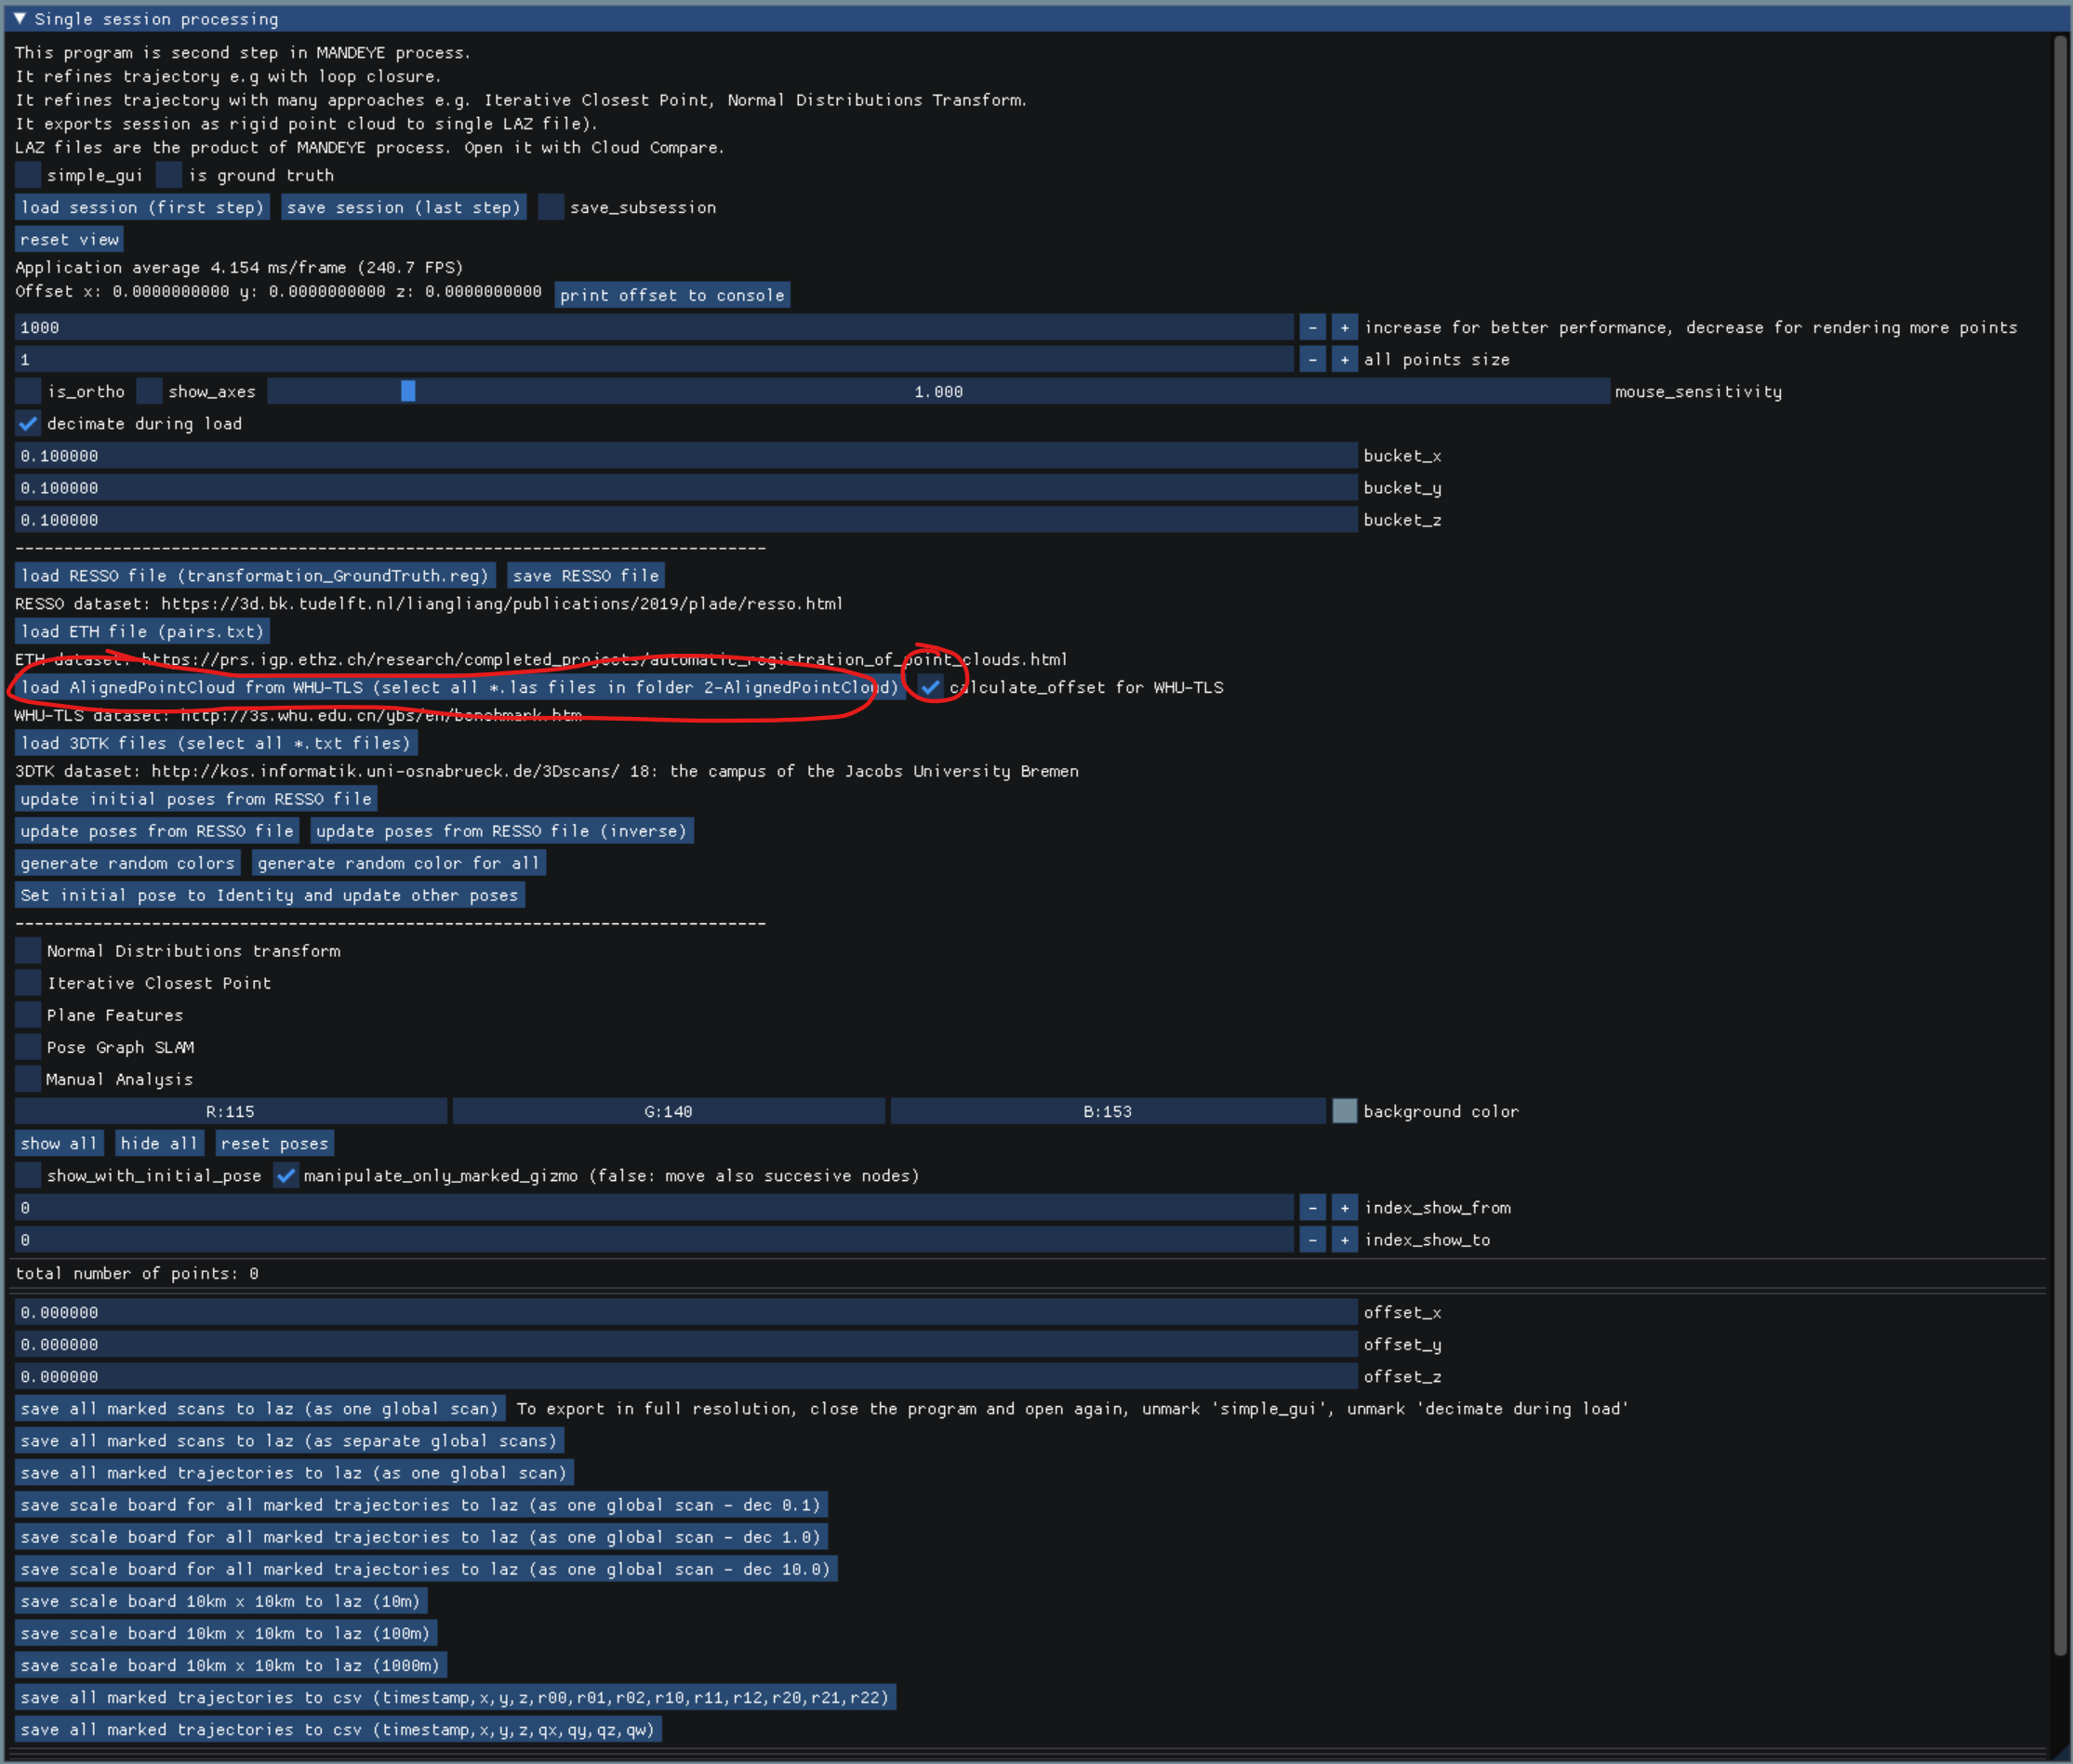
\includegraphics[width=\textwidth]{g2.png}
	\caption{Mark calculate offset for WHU-TLS, load AlignedPointCloud from WHU-TLS (select all *.las/laz files in folder)}
	\label{fig:g2}
\end{figure}

\begin{figure}[H]
	\centering
	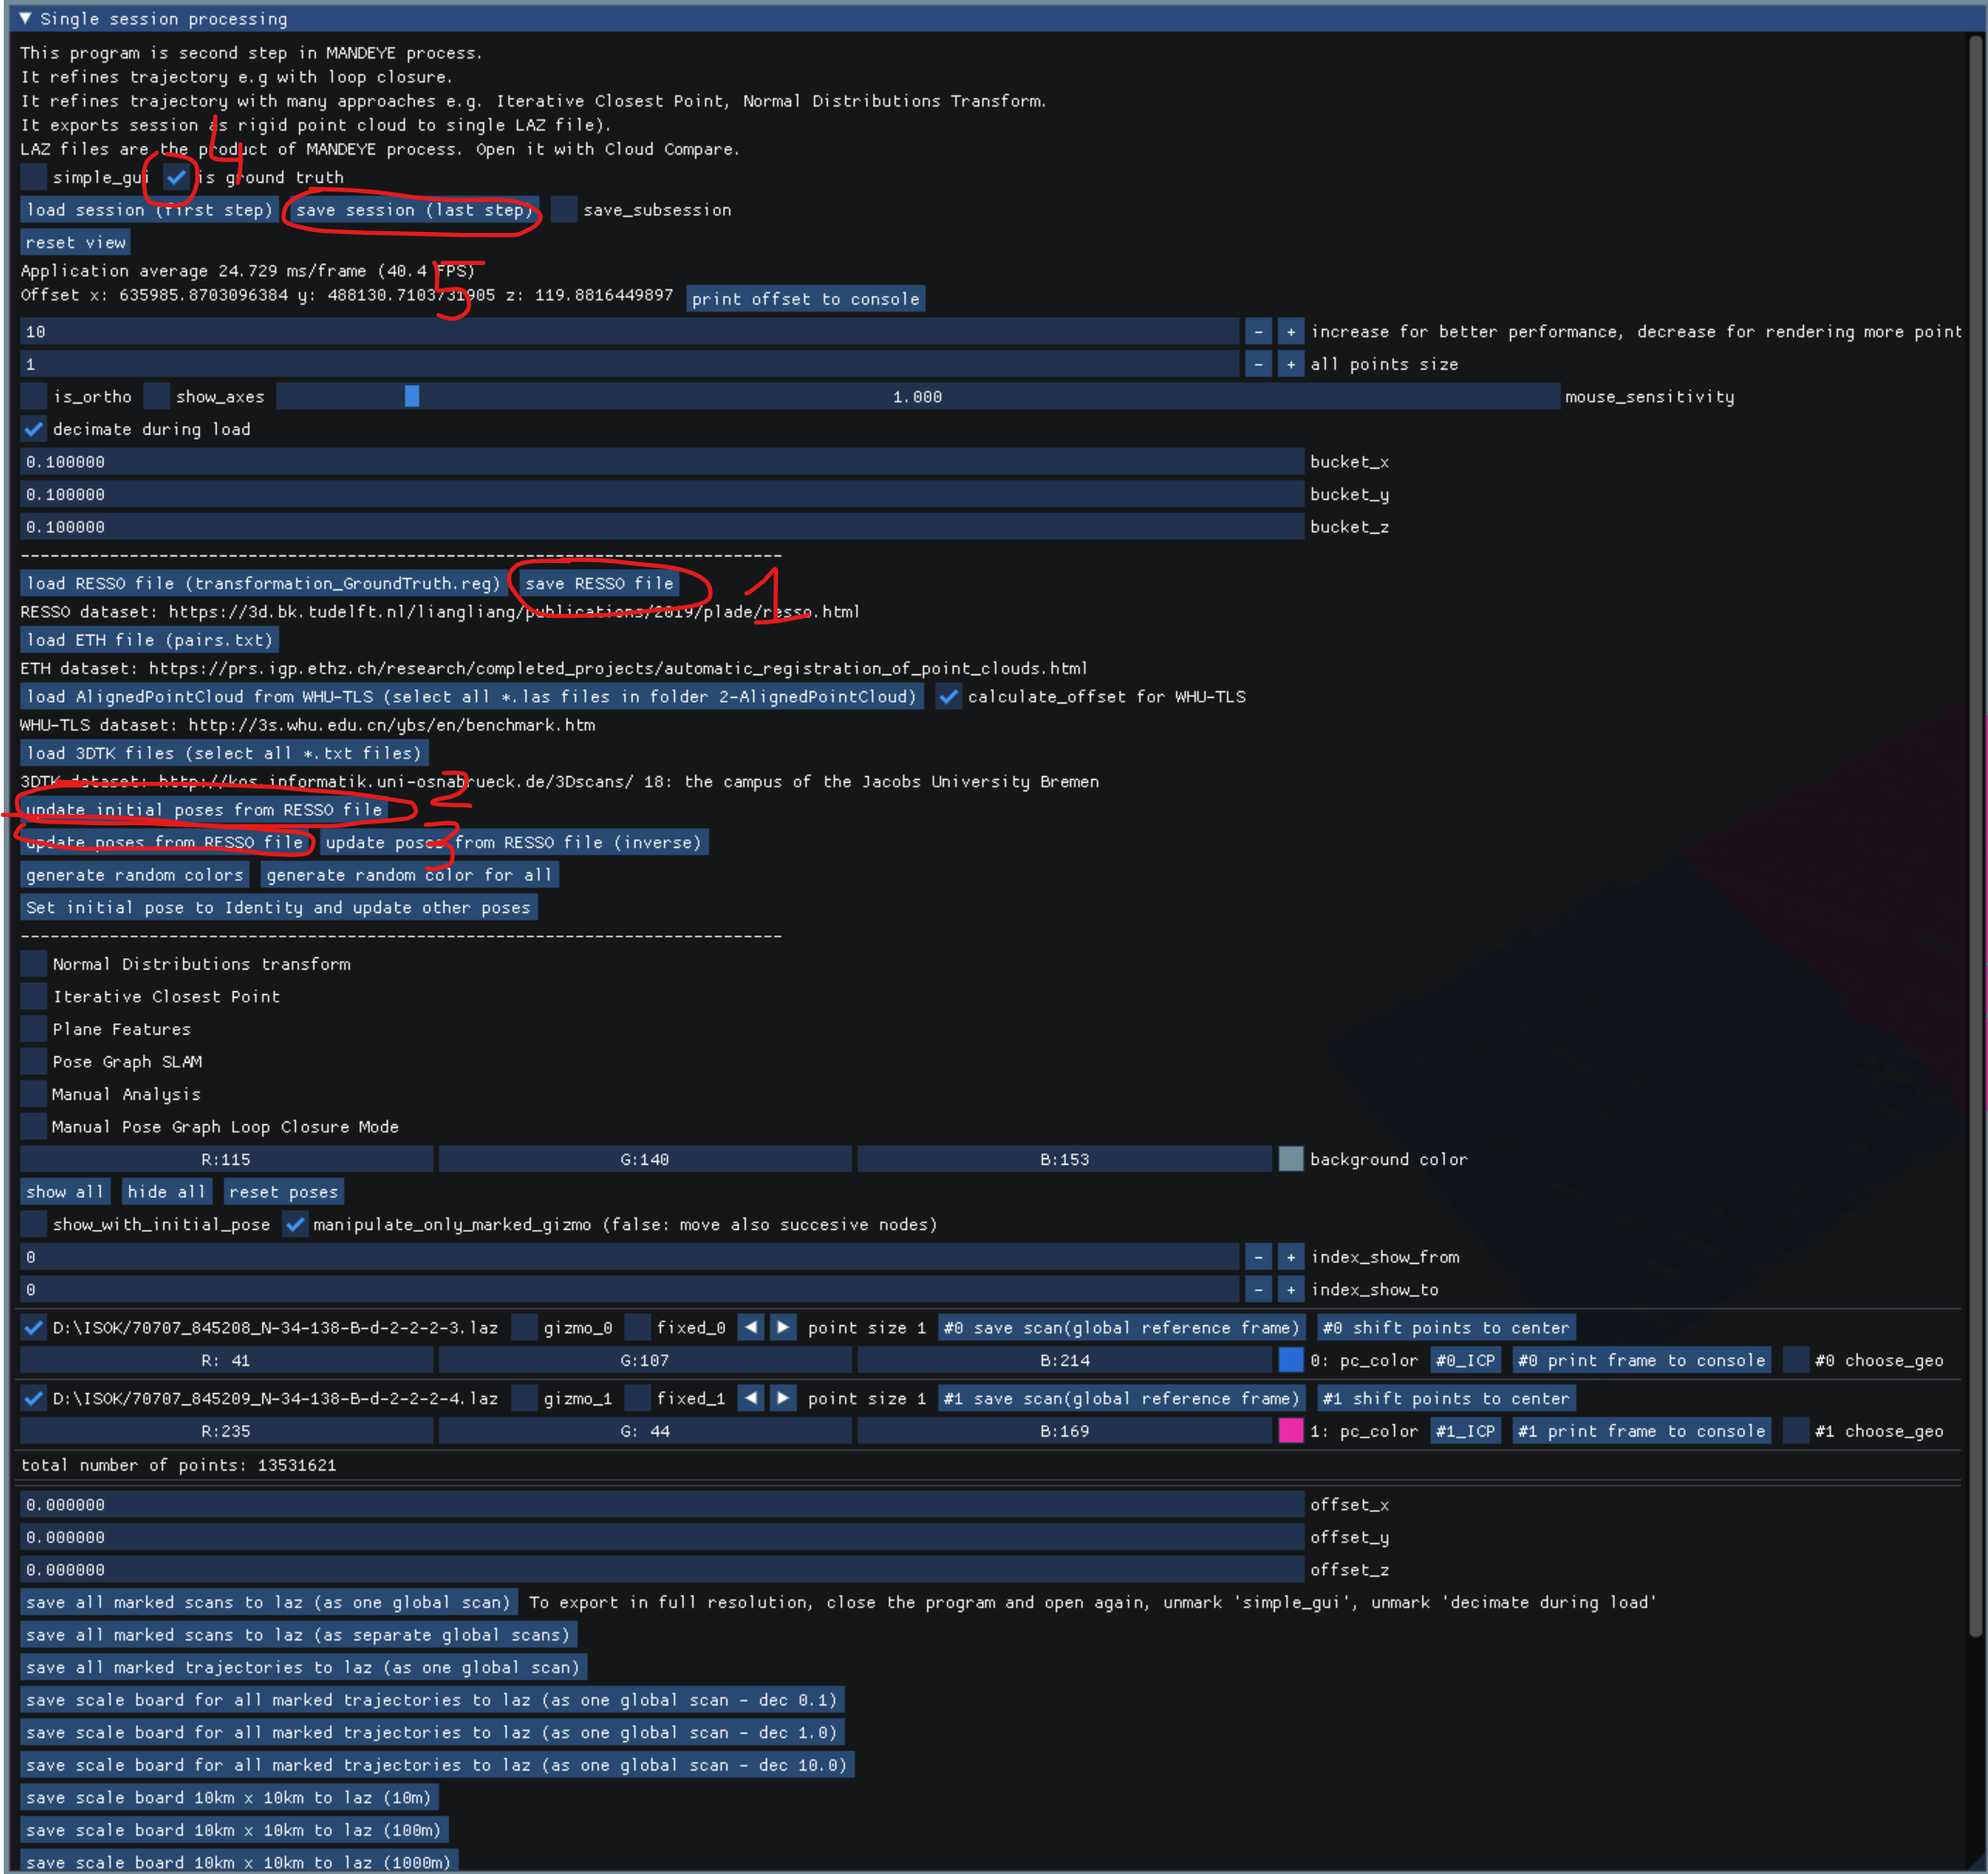
\includegraphics[width=\textwidth]{g3.png}
	\caption{1: save RESSO file, 2: update initial poses from RESSO file (select file from 1), 3: update poses from RESSO file (select file from 1), 4: set checkbox is ground truth, 5: save session.}
	\label{fig:g3}
\end{figure}